%!TEX root = main.tex

\section{Examples of Acceptance-Rejection Reparameterization}
\label{sec:examples}

As two examples, we study rejection sampling and reparameterization of two well-known distributions: the gamma and Dirichlet. These have been widely used as variational families for approximate Bayesian inference. %\cn{Cite something here?} 
We emphasize that \gls{RS-VI} is not limited to these two cases, it applies to any variational family $q(z\g\theta)$ for which a reparameterizable rejection sampler exists. We provide other examples in the supplement.


% ======================================================================
%   EXAMPLE: THE GAMMA DISTRIBUTION
% ======================================================================
\subsection{Gamma Distribution}
\label{subsec:gamma_example}

%An important distribution where rejection sampling is used for simulating random variables is the gamma distribution, $\gam(\alpha,\beta)$, where $\alpha$ is the shape and $\beta$ is the rate. 
One of the most widely used rejection sampler is for the gamma distribution. Indeed, the gamma distribution is also used in practice to generate \eg beta, Dirichlet, and Student's t-distributed random variables. The gamma distribution, $\gam(\alpha,\beta)$, is defined by its shape $\alpha$ and rate $\beta$.

For $\gam(\alpha,1)$ with $\alpha \geq 1$, \citet{Marsaglia:2000} developed an efficient rejection sampler. It uses a truncated version of the following reparameterization
\begin{align}
\label{eq:marsaglia}
  z &= h_{\gam}(\eps,\alpha) \eqdef \left(\alpha-\frac{1}{3}\right)\left(1+\frac{\eps}{\sqrt{9\alpha-3}}\right)^3, \\
\nonumber &\eps \sim s(\eps) \eqdef \N(0,1).%, - \sqrt{9\alpha-3},\infty),
\end{align}
When $\beta \neq 1$, we divide $z$ by the rate $\beta$ and obtain a sample distributed as $\gam(\alpha,\beta)$. The acceptance probability is very high: it exceeds $0.95$ and $0.98$ for $\alpha=1$ and $\alpha=2$, respectively. In fact, as $\alpha \to \infty$ we have that $\pi(\eps\g\theta) \to s(\eps)$, which means that the acceptance probability approaches $1$. Figure~\ref{fig:real_gamma} illustrates the involved functions and distributions for shape $\alpha=2$.

For $\alpha < 1$, we observe that $z = u^{1/\alpha} \tilde z$ is distributed as $\gam(\alpha,\beta)$ for $\tilde z \sim \gam(\alpha+1,\beta)$ and ${u \sim \uni[0,1]}$ \citep{stuart1962,devroye1986}, and apply the rejection sampler above for $\tilde z$.

\begin{figure}[t]
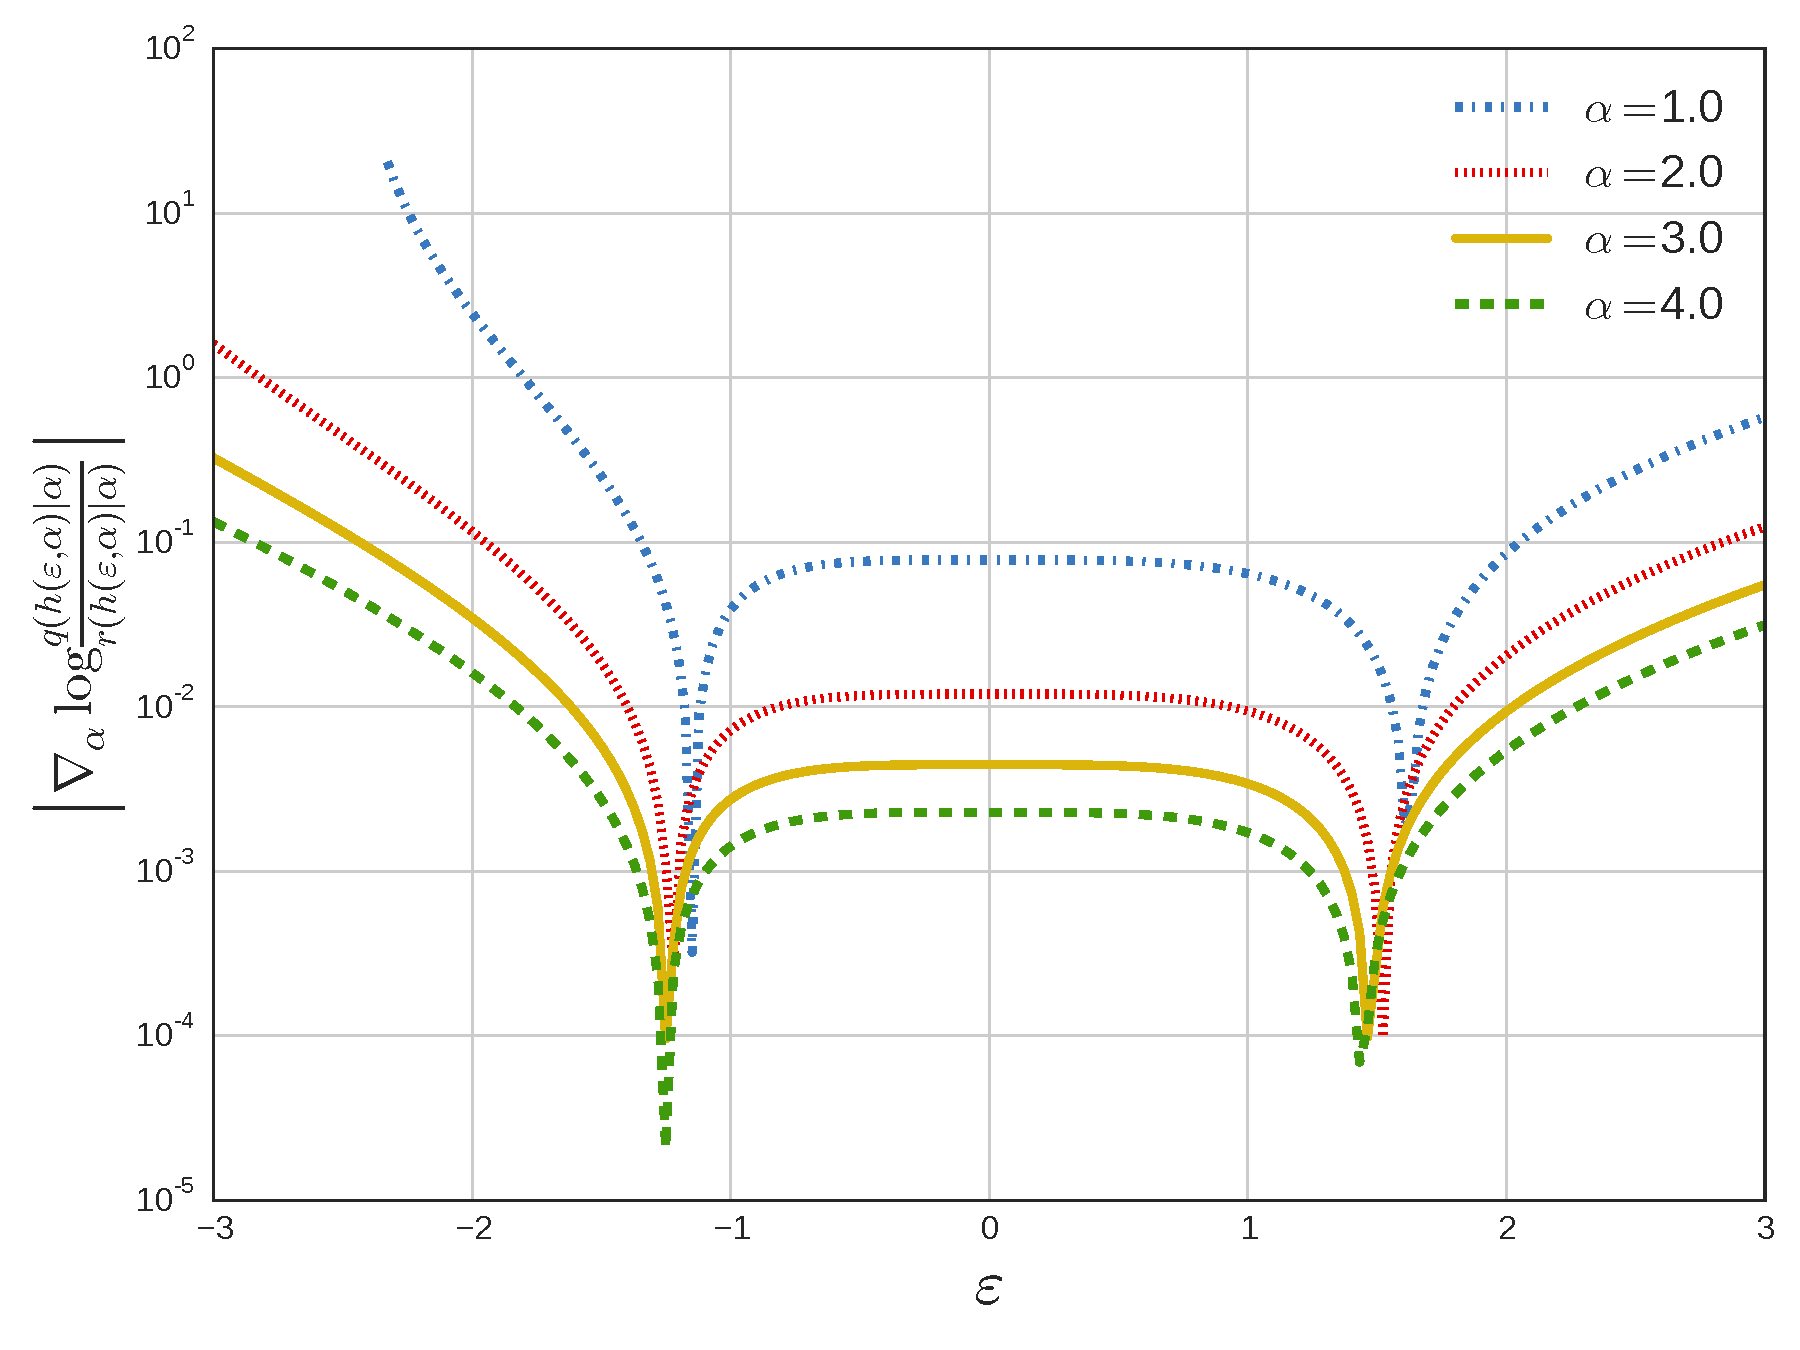
\includegraphics[width=0.9\columnwidth]{correction}
\vspace*{-10pt}
\caption{The correction term of \gls{RS-VI}, and as a result the gradient variance, decreases  with increasing shape $\alpha$. We plot absolute value of the gradient of the log-ratio between the target (gamma) and proposal distributions as a function of $\eps$.% for various settings of shape ($\alpha$).  %\fr{needs a comment about what we want the reader to learn.}
}\label{fig:gammacorr}
\end{figure}

%\cn{Is it interesting to show here that the correction $g_{\text{cor}} \to 0, ~\alpha\to\infty$?}

We now study the quality of the transformation in \eqref{eq:marsaglia} for different values of the shape parameter $\alpha$. Since $\pi(\eps\g\theta) \to s(\eps)$ as $\alpha\to\infty$, we should expect the correction term $g_{\text{cor}}$ to decrease with $\alpha$. We show that in Figure~\ref{fig:gammacorr}, where we plot the log-ratio \eqref{eq:gradQRcorr} from the correction term as a function of $\eps$ for four values of~$\alpha$. We additionally show in Figure~\ref{fig:compare_qeps} that the distribution $\pi(\eps\g\theta)$ converges to $s(\eps)$ (a standard normal) as $\alpha$ increases. For large $\alpha$, $\pi(\eps\g\theta)\approx s(\eps)$ and the acceptance probability of the rejection sampler approaches~$1$, which makes the correction term negligible. In Figure~\ref{fig:compare_qeps}, we also show that $\pi(\eps\g\theta)$ converges faster to a standard normal than the standardization procedure used in \gls{G-REP}. We exploit this property---that performance improves with $\alpha$---to artificially increase the shape for any gamma distribution. We now explain this trick, which we call \emph{shape augmentation}.
\begin{figure*}[t]
  \centering
  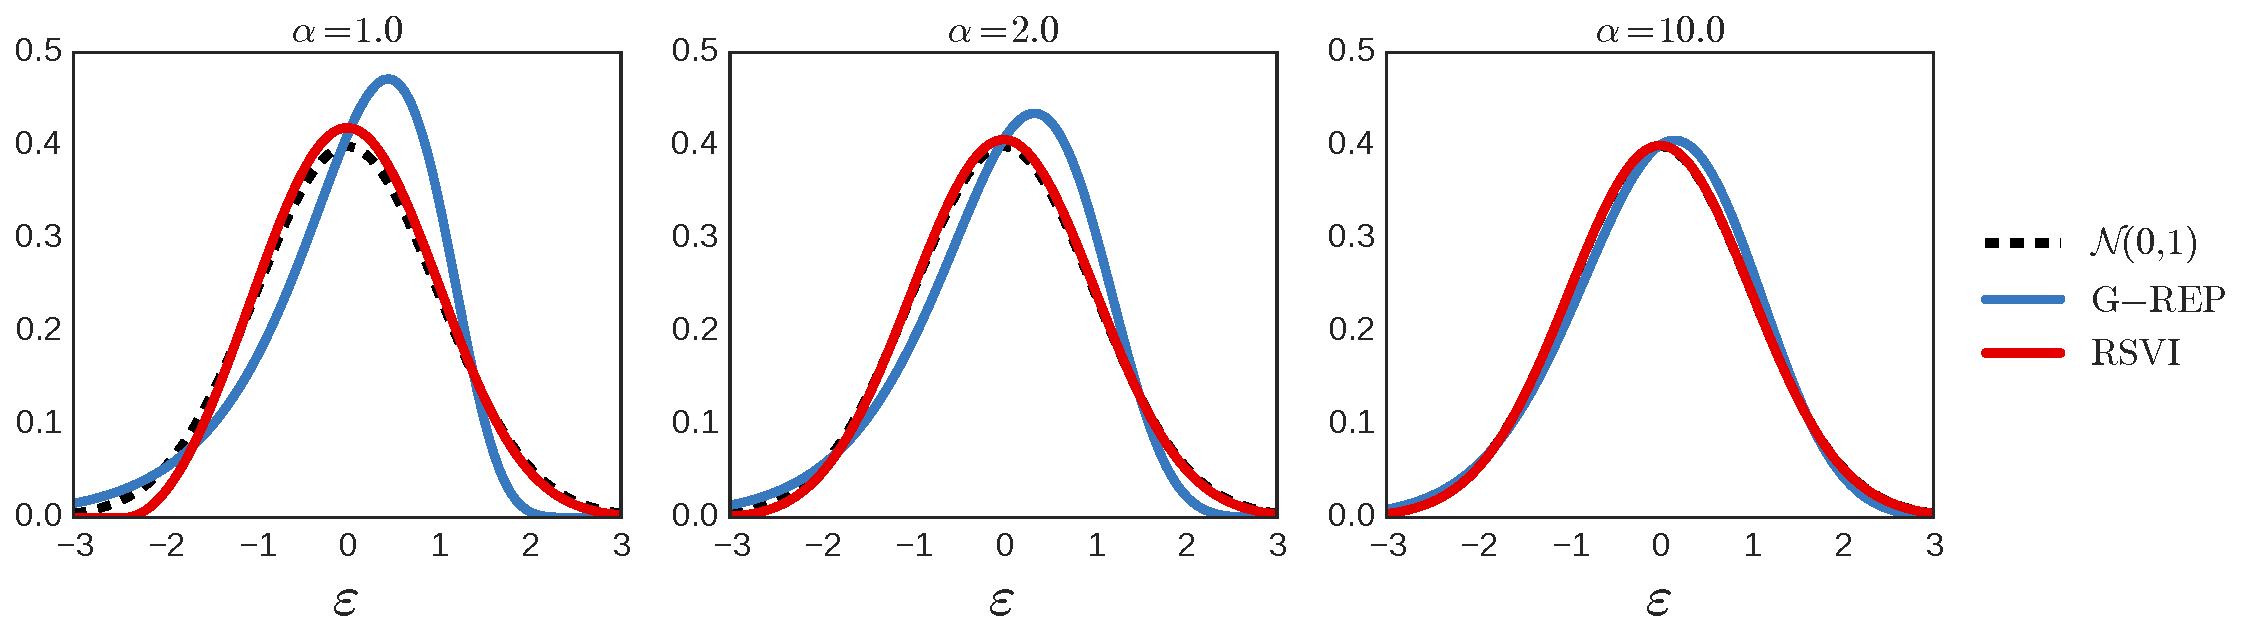
\includegraphics[width=1.5\columnwidth]{compare_Qeps} 
  \vspace*{-10pt}
  \caption{In the distribution on the transformed space $\eps$ for a gamma distribution we can see that the rejection sampling-inspired transformation converges faster to a standard normal. Therefore it is less dependent on the parameter $\alpha$, which implies a smaller correction term. We compare the transformation of \gls{RS-VI} (this paper) with the standardization procedure suggested in \gls{G-REP} \citep{RuizTB2016}, for shape parameters $\alpha = \{1,2,10\}$.}
  %\caption{Distribution on the transformed space $\eps$ for a gamma distribution with shape parameter $\alpha = \{1,2,10\}$. We compare the transformation of our reparameterized rejection sampler with the standardization procedure suggested in \gls{G-REP} \citep{RuizTB2016}. The transformation inspired by rejection sampling converges faster to a standard normal, and therefore it is less dependent on the parameter $\alpha$, which implies a smaller correction term.}
  \label{fig:compare_qeps}
\end{figure*}

%how the gradient of the log-ratio \eqref{eq:gradQRcorr} from the correction term varies as a function of $\eps$ for several values of $\alpha$. As $\alpha$ increases, the log-ratio decreases and thus $g_{\text{cor}}$ will also decrease. Below we show how we can control the shape targeted by the rejection sampler by repeated use of the above trick with uniforms. Below we show how we can control the shape targeted by the rejection sampler by repeated use of the above trick with uniforms.

\parhead{Shape augmentation.}
Here we show how to exploit the fact that the rejection sampler improves for increasing shape $\alpha$. We make repeated use of the trick above, using uniform variables, to control the value of $\alpha$ that goes into the rejection sampler. That is, to compute the \gls{ELBO} for a $\gam(\alpha,1)$ distribution, we can first express the random variable as $z = \tilde z \prod_{i=1}^B u_i^{\frac{1}{\alpha+i-1}}$ (for some positive integer $B$), $\tilde z \sim \gam(\alpha+B,1)$ and $u_i \iidsim \uni[0,1]$. This can be proved by induction, since $\tilde z u_B^{\frac{1}{\alpha+B-1}} \sim \gam(\alpha+B-1,1)$, $\tilde z u_B^{\frac{1}{\alpha+B-1}} u_{B-1}^{\frac{1}{\alpha+B-2}} \sim \gam(\alpha+B-2,1)$, \etc. Hence, we can apply the rejection sampling framework for $\tilde z \sim \gam(\alpha+B,1)$ instead of the original $z$. We study the effect of shape augmentation on the variance in Section~\ref{subsec:dirichlet_example}.
%More details are provided in the Supplementary material. 
%\cn{Plot and discussion here regarding $I_k$ and dependence on $\theta$?}


% ======================================================================
%   EXAMPLE: THE DIRICHLET DISTRIBUTION
% ======================================================================
\subsection{Dirichlet Distribution}
\label{subsec:dirichlet_example}

The $\diri(\alpha_{1:K})$ distribution, with concentration parameters $\alpha_{1:K}$, is a $K$-dimensional multivariate distribution with ${K-1}$ degrees of freedom. To simulate random variables we use the fact that if ${\tilde z_k \sim \gam(\alpha_k,1)}$ \iid, then ${z_{1:K} = \left(\sum_\ell \tilde z_\ell\right)^{-1}(\tilde z_1,\ldots,\tilde z_K)^\top \sim \diri(\alpha_{1:K})}$. 

Thus, we make a change of variables to reduce the problem to that of simulating independent gamma distributed random variables,
\begin{align*}
&\E_{q(z_{1:K}\g\alpha_{1:K})}[f(z_{1:K})] =\\
&= \int f\left( \frac{\tilde z_{1:K}}{\sum_{\ell=1}^K \tilde z_\ell}\right)\prod_{k=1}^K\gam(\tilde z_k\g\alpha_k,1) \myd \tilde z_{1:K}.
\end{align*}
We apply the transformation in Section~\ref{subsec:gamma_example} for the gamma-distributed variables, $\tilde z_k = h_{\gam}(\eps_k,\alpha_k)$, where the variables $\eps_k$ are generated by independent gamma rejection samplers.
\begin{figure}[t]
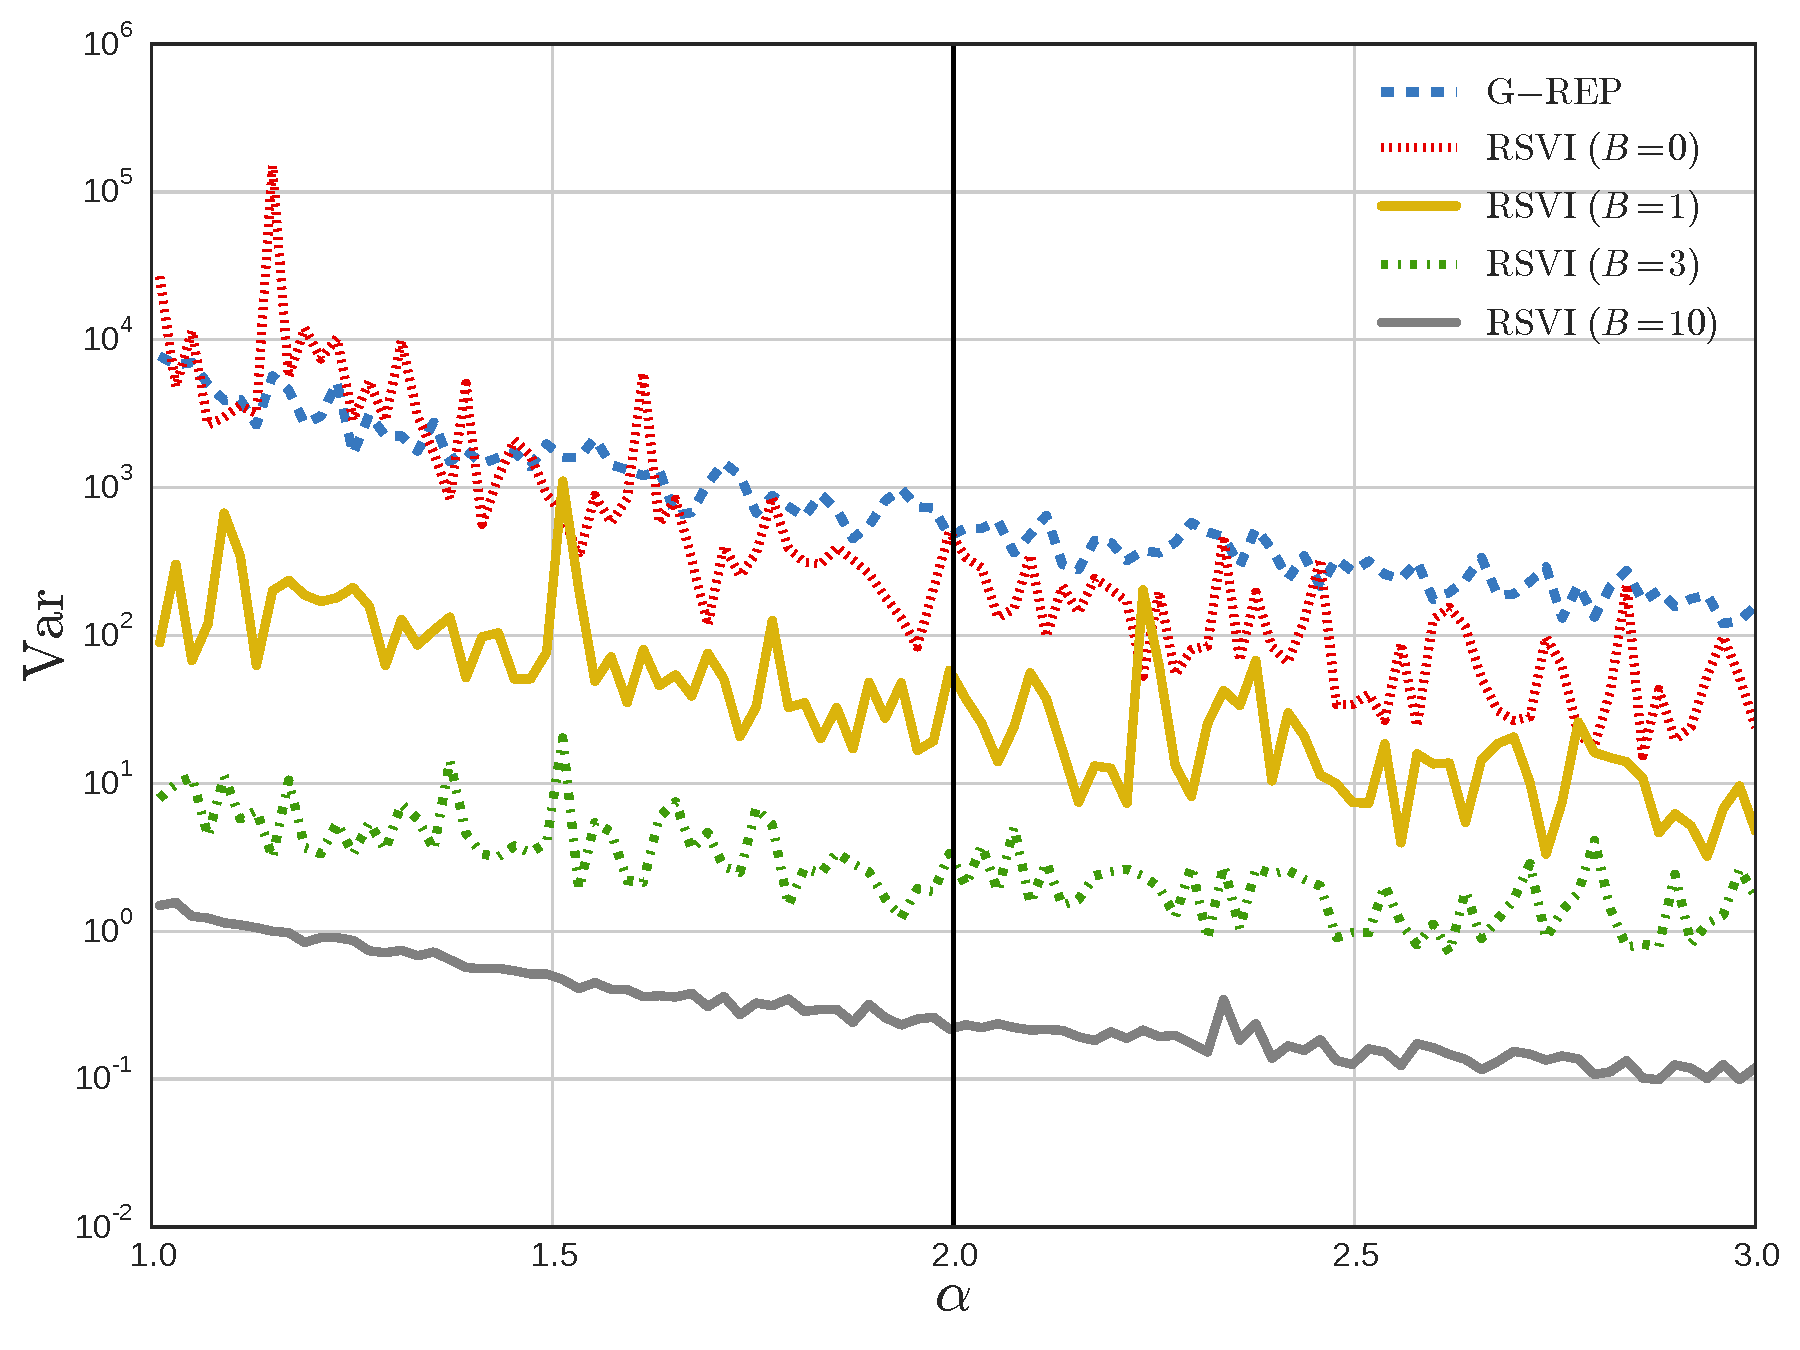
\includegraphics[width=0.9\columnwidth]{dirichletN100K100}
\caption{\gls{RS-VI} (this paper) achieves lower variance compared to \gls{G-REP} \citep{RuizTB2016}. The estimated variance is for the first component of Dirichlet approximation to a multinomial likelihood with uniform Dirichlet prior.  Optimal concentration is $\alpha=2$, and $B$ denotes shape augmentation. %\fr{remove details which are in main text; add ideas that we want to convey}
}\label{fig:dirichlet}
\end{figure}
To showcase this, we study a simple conjugate model where the exact gradient and posterior are available: a multinomial likelihood with Dirichlet prior and Dirichlet variational distribution. In Figure~\ref{fig:dirichlet} we show the resulting variance of the first component of the gradient, based on simulated data from a Dirichlet distribution with $K=100$ components, uniform prior, and $N=100$ trials. We compare the variance of \gls{RS-VI} (for various shape augmentation settings) with the \gls{G-REP} approach \citep{RuizTB2016}. \gls{RS-VI} performs better even without the augmentation trick, and significantly better with it.


%This enables the following reparameterization for the Dirichlet distribution
%\begin{align*}
%&z_{1:K} = \left( \bar h_{\gam}(\eps_1,\alpha_1),\ldots,\bar h_{\gam}(\eps_K,\alpha_K)\right)^\top, \\
%&\bar h_{\gam}(\eps_k,\alpha_k) = \frac{h_{\gam}(\eps_k,\alpha_k)}{\sum_{\ell=1}^K h_{\gam}(\eps_\ell,\alpha_\ell)},\\
%&\eps_k \iidsim s(\eps) \eqdef \N(0,1),
%\end{align*}
%where $\eps_{1:K}$ are obtained by running $K$ independent rejection samplers for $\gam(\alpha_k,1), ~k=1,\ldots,K$, respectively. 

% ======================================================================
%   EXAMPLE: THE BETA DISTRIBUTION
% ======================================================================
%\subsubsection*{Beta Distribution}
%The beta distribution, $\bet(\alpha,\beta)$, is characterized by its two shape parameters $\alpha$ and $\beta$. A simple and efficient way is to generate two independen random variables $\bar z \sim \gam(\alpha,1)$, $\tilde z \sim \gam(\beta,1)$, and then $z = \frac{\bar z}{\bar z + \tilde z} \sim \bet(\alpha,\beta)$. This means we can make use of two independent rejection samplers generating $\eps_1$ for $\gam(\alpha,1)$, $\eps_2$ for $\gam(\beta,1)$, and let
%\begin{align*}
%&h_{\bet}(\eps_{1:2},\alpha,\beta) = \frac{h_{\gam}(\eps_{1},\alpha)}{h_{\gam}(\eps_{1},\alpha)+h_{\gam}(\eps_{2},\beta)},\\
%&\eps_1,\eps_2 \sim \N(0,1).
%\end{align*}
%Note that here it is important to take into account that $\eps_1$ and $\eps_2$ correspond to two \emph{independent} rejection samplers, which means we do not have to propose $\eps_{1:2}$ jointly. We thus get $\pi(\eps_\tau,u_\tau) = \pi(\eps_{\tau_1},u_{\tau_1})\pi(\eps_{\tau_2},u_{\tau_2})$, where $\tau_i$ indicates final iteration for rejection sampler number~$i$. The correction term is given as follows
%\begin{align*}
%g_{\text{cor}}=\E_{\pi(\eps_\tau,u_\tau)}&\Bigg[f(h_{\bet}(\eps_\tau,\alpha,\beta))\\
%&\left.\quad \cdot
%\left(
%\begin{array}{c}
%\frac{\myd}{\myd \alpha} \log \frac{q_\alpha(h_{\gam}(\eps_{\tau_1},\alpha))}{r_\alpha(h_{\gam}(\eps_{\tau_1},\alpha))} \\
%\frac{\myd}{\myd \beta}\log \frac{q_\beta(h_{\gam}(\eps_{\tau_2},\beta))}{r_\beta(h_{\gam}(\eps_{\tau_2},\beta))}
%\end{array}
%\right)\right],
%\end{align*}
%where $q_{\alpha/\beta}(z), r_{\alpha/\beta}(z)$ is the standard proposal and target in the Gamma rejection sampler with shape $\alpha/\beta$, respectively. The above procedure generalizes straightforwardly to the Dirichlet distribution because $z=\left(\sum_\ell \tilde z_\ell\right)^{-1}\cdot (\tilde z_1,\ldots,\tilde z_K)^\top \sim \diri(K,\alpha_{1:K})$ for $\tilde z_k \sim \gam(\alpha_k,1)$.

%When $\alpha,\beta > 1$ the beta distribution is finite on its support and we could potentially design a rejection sampler based on the uniform distribution, \ie ${h_{\bet}(\eps,\alpha,\beta ) = \eps, ~ \eps\sim\uni[0,1]}$. This rejection sampler would of course be very inefficient with low acceptance probability. Furthermore, $g_{\text{rep}} \equiv 0$ and $g_{\text{cor}} = \E_{\pi(\eps_\tau,u_\tau)}\left[f(\eps_\tau) \grad_\theta \log q_\theta(\eps_\tau)\right]$. We can see that this in fact gives us back the traditional score function estimator because $\eps_\tau \sim \bet(\alpha,\beta)$. This shows us that it is important to design an efficient rejection sampler so that the correction term, $g_{\text{cor}}$, is small.
%For details on how we deal with Beta and Dirichlet distributions see the Supplementary material.
%\subsubsection*{Dirichlet Distribution}
%For a Dirichled distribution with $K$ components and $\alpha_{1:K}$ concentration parameters we can simulate by making use of the Gamma rejection sampler. Given $\tilde z \sim \prod_{k=1}^K \G(\alpha_k,1)$, we can obtain a Dirichlet-distributed random variable by normalizing $\tilde z$, \ie dividing each component with the total sum.
%\begin{align*}
%z &= h_{\text{D}}(\eps^{1:K},\alpha_{1:K}) \eqdef \frac{1}{\sum_\ell h_\gamma(\eps^\ell,\alpha_\ell,1)}
%\left(
%\begin{array}{c}
%h_\gamma(\eps^1,\alpha_1,1)\\
%\vdots\\
%h_\gamma(\eps^K,\alpha_K,1)
%\end{array}
%\right)
%\end{align*}
%\subsubsection*{Von Mises Distribution}
